\documentclass[]{article}
\usepackage{lmodern}
\usepackage{amssymb,amsmath}
\usepackage{ifxetex,ifluatex}
\usepackage{fixltx2e} % provides \textsubscript
\ifnum 0\ifxetex 1\fi\ifluatex 1\fi=0 % if pdftex
  \usepackage[T1]{fontenc}
  \usepackage[utf8]{inputenc}
\else % if luatex or xelatex
  \ifxetex
    \usepackage{mathspec}
    \usepackage{xltxtra,xunicode}
  \else
    \usepackage{fontspec}
  \fi
  \defaultfontfeatures{Mapping=tex-text,Scale=MatchLowercase}
  \newcommand{\euro}{€}
\fi
% use upquote if available, for straight quotes in verbatim environments
\IfFileExists{upquote.sty}{\usepackage{upquote}}{}
% use microtype if available
\IfFileExists{microtype.sty}{%
\usepackage{microtype}
\UseMicrotypeSet[protrusion]{basicmath} % disable protrusion for tt fonts
}{}
\usepackage[margin=1in]{geometry}
\usepackage{color}
\usepackage{fancyvrb}
\newcommand{\VerbBar}{|}
\newcommand{\VERB}{\Verb[commandchars=\\\{\}]}
\DefineVerbatimEnvironment{Highlighting}{Verbatim}{commandchars=\\\{\}}
% Add ',fontsize=\small' for more characters per line
\usepackage{framed}
\definecolor{shadecolor}{RGB}{248,248,248}
\newenvironment{Shaded}{\begin{snugshade}}{\end{snugshade}}
\newcommand{\KeywordTok}[1]{\textcolor[rgb]{0.13,0.29,0.53}{\textbf{{#1}}}}
\newcommand{\DataTypeTok}[1]{\textcolor[rgb]{0.13,0.29,0.53}{{#1}}}
\newcommand{\DecValTok}[1]{\textcolor[rgb]{0.00,0.00,0.81}{{#1}}}
\newcommand{\BaseNTok}[1]{\textcolor[rgb]{0.00,0.00,0.81}{{#1}}}
\newcommand{\FloatTok}[1]{\textcolor[rgb]{0.00,0.00,0.81}{{#1}}}
\newcommand{\CharTok}[1]{\textcolor[rgb]{0.31,0.60,0.02}{{#1}}}
\newcommand{\StringTok}[1]{\textcolor[rgb]{0.31,0.60,0.02}{{#1}}}
\newcommand{\CommentTok}[1]{\textcolor[rgb]{0.56,0.35,0.01}{\textit{{#1}}}}
\newcommand{\OtherTok}[1]{\textcolor[rgb]{0.56,0.35,0.01}{{#1}}}
\newcommand{\AlertTok}[1]{\textcolor[rgb]{0.94,0.16,0.16}{{#1}}}
\newcommand{\FunctionTok}[1]{\textcolor[rgb]{0.00,0.00,0.00}{{#1}}}
\newcommand{\RegionMarkerTok}[1]{{#1}}
\newcommand{\ErrorTok}[1]{\textbf{{#1}}}
\newcommand{\NormalTok}[1]{{#1}}
\usepackage{graphicx}
\makeatletter
\def\maxwidth{\ifdim\Gin@nat@width>\linewidth\linewidth\else\Gin@nat@width\fi}
\def\maxheight{\ifdim\Gin@nat@height>\textheight\textheight\else\Gin@nat@height\fi}
\makeatother
% Scale images if necessary, so that they will not overflow the page
% margins by default, and it is still possible to overwrite the defaults
% using explicit options in \includegraphics[width, height, ...]{}
\setkeys{Gin}{width=\maxwidth,height=\maxheight,keepaspectratio}
\ifxetex
  \usepackage[setpagesize=false, % page size defined by xetex
              unicode=false, % unicode breaks when used with xetex
              xetex]{hyperref}
\else
  \usepackage[unicode=true]{hyperref}
\fi
\hypersetup{breaklinks=true,
            bookmarks=true,
            pdfauthor={},
            pdftitle={},
            colorlinks=true,
            citecolor=blue,
            urlcolor=blue,
            linkcolor=magenta,
            pdfborder={0 0 0}}
\urlstyle{same}  % don't use monospace font for urls
\setlength{\parindent}{0pt}
\setlength{\parskip}{6pt plus 2pt minus 1pt}
\setlength{\emergencystretch}{3em}  % prevent overfull lines
\setcounter{secnumdepth}{0}

%%% Change title format to be more compact
\usepackage{titling}
\setlength{\droptitle}{-2em}
  \title{}
  \pretitle{\vspace{\droptitle}}
  \posttitle{}
  \author{}
  \preauthor{}\postauthor{}
  \date{}
  \predate{}\postdate{}

\newcommand{\beginsupplement}{%
        \setcounter{table}{0}
        \renewcommand{\thetable}{S\arabic{table}}%
        \setcounter{figure}{0}
        \renewcommand{\thefigure}{S\arabic{figure}}%
     }

\begin{document}

\maketitle


\section{\texorpdfstring{Example analyses of autotetraploid potato
(\emph{Solanum
tuberosum})}{Example analyses of autotetraploid potato (Solanum tuberosum)}}\label{example-analyses-of-autotetraploid-potato-solanum-tuberosum}

The following walk-through will take you through every step of analyzing
the data set for autotetraploid potato (\emph{Solanum tuberosum}) that
was completed in the manuscript. Because the analysis with
\textsc{polyfreqs} takes a few hours (there are 86,400 parameters to
estimate), we have provided the output from that step for you. The
potato data set is provided for free with the R package
\textsc{fitTetra}, and the code below goes through how we acquired and
reformatted it for an analysis with \textsc{polyfreqs}. Instructions for
installing \textsc{polyfreqs} can be found on the GitHub page associated
with the package (\url{https://github.com/pblischak/polyfreqs}). The
following sections are intended to be completed with the data in the
\texttt{example/} folder accompanying the manuscript found on GitHub
(\url{https://github.com/pblischak/polyfreqs-ms-data}).

\begin{Shaded}
\begin{Highlighting}[]
\CommentTok{# Using autetraploid potato data from the fitTetra package.}
\CommentTok{#}
\CommentTok{# If not installed, install it using:}
\CommentTok{# install.packages("fitTetra")}
\CommentTok{#}
\CommentTok{# Then load the data.}
\KeywordTok{library}\NormalTok{(fitTetra)}
\KeywordTok{data}\NormalTok{(tetra.potato.SNP)}

\CommentTok{# Get the names of the individuals and loci.}
\NormalTok{samples <-}\StringTok{ }\KeywordTok{unique}\NormalTok{(tetra.potato.SNP$SampleName)}
\NormalTok{markers <-}\StringTok{ }\KeywordTok{unique}\NormalTok{(tetra.potato.SNP$MarkerName)}

\CommentTok{# Initialize x and y matrices -- x will be the reference allele.}
\NormalTok{potato_mat_x <-}\StringTok{ }\KeywordTok{matrix}\NormalTok{(}\OtherTok{NA}\NormalTok{, }\DataTypeTok{nrow=}\KeywordTok{length}\NormalTok{(}\KeywordTok{unique}\NormalTok{(tetra.potato.SNP$SampleName)), }
                       \DataTypeTok{ncol=}\KeywordTok{length}\NormalTok{(}\KeywordTok{unique}\NormalTok{(tetra.potato.SNP$MarkerName)))}
\KeywordTok{rownames}\NormalTok{(potato_mat_x) <-}\StringTok{ }\NormalTok{samples}
\KeywordTok{colnames}\NormalTok{(potato_mat_x) <-}\StringTok{ }\NormalTok{markers}

\NormalTok{potato_mat_y <-}\StringTok{ }\KeywordTok{matrix}\NormalTok{(}\OtherTok{NA}\NormalTok{, }\DataTypeTok{nrow=}\KeywordTok{length}\NormalTok{(}\KeywordTok{unique}\NormalTok{(tetra.potato.SNP$SampleName)), }
                       \DataTypeTok{ncol=}\KeywordTok{length}\NormalTok{(}\KeywordTok{unique}\NormalTok{(tetra.potato.SNP$MarkerName)))}

\CommentTok{# Get the counts from the data frame.}
\NormalTok{for(i in }\DecValTok{1}\NormalTok{:}\KeywordTok{dim}\NormalTok{(potato_mat_x)[}\DecValTok{1}\NormalTok{])\{}
    \NormalTok{tmp <-}\StringTok{ }\KeywordTok{subset}\NormalTok{(tetra.potato.SNP, SampleName==samples[i])}
    \NormalTok{potato_mat_x[i,] <-}\StringTok{ }\NormalTok{tmp$X_Raw}
    \NormalTok{potato_mat_y[i,] <-}\StringTok{ }\NormalTok{tmp$Y_Raw}
\NormalTok{\}}

\CommentTok{# Get the total counts as the sum of x and y and give row and column names.}
\NormalTok{potato_mat_tot <-}\StringTok{ }\NormalTok{potato_mat_x +}\StringTok{ }\NormalTok{potato_mat_y}
\KeywordTok{rownames}\NormalTok{(potato_mat_tot) <-}\StringTok{ }\NormalTok{samples}
\KeywordTok{colnames}\NormalTok{(potato_mat_tot) <-}\StringTok{ }\NormalTok{markers}

\CommentTok{# Rescale, then print the tables to file in a format suitable for polyfreqs.}

\NormalTok{potato_mat_x <-}\StringTok{ }\KeywordTok{round}\NormalTok{(potato_mat_x/}\DecValTok{100}\NormalTok{)}
\NormalTok{potato_mat_tot <-}\StringTok{ }\KeywordTok{round}\NormalTok{(potato_mat_tot/}\DecValTok{100}\NormalTok{)}

\KeywordTok{write.table}\NormalTok{(potato_mat_x, }\DataTypeTok{file=}\StringTok{"potato_ref_reads.txt"}\NormalTok{, }\DataTypeTok{quote=}\NormalTok{F, }\DataTypeTok{sep=}\StringTok{"}\CharTok{\textbackslash{}t}\StringTok{"}\NormalTok{)}
\KeywordTok{write.table}\NormalTok{(potato_mat_tot, }\DataTypeTok{file=}\StringTok{"potato_tot_reads.txt"}\NormalTok{, }\DataTypeTok{quote=}\NormalTok{F, }\DataTypeTok{sep=}\StringTok{"}\CharTok{\textbackslash{}t}\StringTok{"}\NormalTok{)}
\end{Highlighting}
\end{Shaded}

\newpage

If you look at the files that we just wrote
(\texttt{potato\_ref\_reads.txt} and \texttt{potato\_tot\_reads.txt}),
you can see how data should be formatted for running an analysis with
\textsc{polyfreqs}. More details will be provided in the next section
when we read in the data and analyze it.

\subsection{\texorpdfstring{\emph{Calculating expected and observed
heterozygosity}}{Calculating expected and observed heterozygosity}}\label{calculating-expected-and-observed-heterozygosity}

Next we will read the data into R. The simplest way to do this is to use
the \texttt{read.table()} function. In the total and reference read
count files for the potato data, the first row is a tab delimited list
of locus names. This row is optional and can be excluded. After that,
each row has the name of the individual followed by the read counts at
each locus (tab delimited). The individual name is required because it
is used when writing genotype samples to file (set \texttt{genotypes=T}
when running \textsc{polyfreqs}). To specify that the first column
contains the names, we use the \texttt{row.names} argument and set it
equal to 1. To specify that the first row has column names for each
locus (you don't need a label for the names), set the \texttt{header}
argument to \texttt{TRUE}. With the data read in, all that is left to do
is to load \textsc{polyfreqs} and set up an analysis.

\begin{quote}
\textbf{NB}: When the data are passed to the \texttt{polyfreqs()}
function, make sure that they are converted to matrices using the
\texttt{as.matrix()} function.
\end{quote}

\begin{Shaded}
\begin{Highlighting}[]
\CommentTok{# Read in data using read.table. Remember the row.names and header options.}
\CommentTok{# If you don't have locus names in the first row, take out header=T.}
\NormalTok{potato_tot_table <-}\StringTok{ }\KeywordTok{read.table}\NormalTok{(}\StringTok{"potato_tot_reads.txt"}\NormalTok{, }\DataTypeTok{row.names=}\DecValTok{1}\NormalTok{, }\DataTypeTok{header=}\NormalTok{T)}
\NormalTok{potato_ref_table <-}\StringTok{ }\KeywordTok{read.table}\NormalTok{(}\StringTok{"potato_ref_reads.txt"}\NormalTok{, }\DataTypeTok{row.names=}\DecValTok{1}\NormalTok{, }\DataTypeTok{header=}\NormalTok{T)}

\CommentTok{# Load polyfreqs}
\KeywordTok{library}\NormalTok{(polyfreqs)}

\CommentTok{# Run through polyfreqs with genotypes=T}
\CommentTok{# and geno_dir="./potato_genotypes/".}
\CommentTok{# Make sure you use the as.matrix() command.}
\NormalTok{potato_out <-}\StringTok{ }\KeywordTok{polyfreqs}\NormalTok{(}\KeywordTok{as.matrix}\NormalTok{(potato_tot_table), }
                        \KeywordTok{as.matrix}\NormalTok{(potato_ref_table), }\DataTypeTok{ploidy=}\DecValTok{4}\NormalTok{, }\DataTypeTok{iter=}\DecValTok{100000}\NormalTok{, }
                        \DataTypeTok{genotypes=}\NormalTok{T, }\DataTypeTok{geno_dir=}\StringTok{"potato_genotypes"}\NormalTok{, }
                        \DataTypeTok{outfile=}\StringTok{"potato_mcmc.out"}\NormalTok{)}
\end{Highlighting}
\end{Shaded}

The \texttt{potato\_out} object will be a list of four items:

\begin{itemize}
\item
  \texttt{potato\_out\$posterior\_freqs} -- a matrix of the posterior
  samples of allele frequencies at each locus prior to burn-in (also
  printed to the file \texttt{potato\_mcmc.out}).
\item
  \texttt{potato\_out\$map\_genotypes} -- a matrix of the maximum
  \emph{a posteriori} genotypes for each individual at each locus
  estimated using the posterior mode.
\item
  \texttt{potato\_out\$het\_obs} -- a matrix of the per locus posterior
  samples of observed heterozygosity.
\item
  \texttt{potato\_out\$het\_exp} -- a matrix of the per locus posterior
  samples of expected heterozygosity.
\end{itemize}

We will write each of these to file for downstream analyses.

\begin{Shaded}
\begin{Highlighting}[]
\KeywordTok{write.table}\NormalTok{(potato_out$map_genotypes, }\StringTok{"potato_map_genotypes.txt"}\NormalTok{, }\DataTypeTok{quote=}\NormalTok{F, }
            \DataTypeTok{row.names=}\NormalTok{F, }\DataTypeTok{col.names=}\NormalTok{F)}
\KeywordTok{write.table}\NormalTok{(potato_out$het_obs, }\StringTok{"potato_het_obs.txt"}\NormalTok{, }\DataTypeTok{quote=}\NormalTok{F, }
            \DataTypeTok{row.names=}\NormalTok{F, }\DataTypeTok{col.names=}\NormalTok{F)}
\KeywordTok{write.table}\NormalTok{(potato_out$het_exp, }\StringTok{"potato_het_exp.txt"}\NormalTok{, }\DataTypeTok{quote=}\NormalTok{F, }
            \DataTypeTok{row.names=}\NormalTok{F, }\DataTypeTok{col.names=}\NormalTok{F)}\ErrorTok{)}
\end{Highlighting}
\end{Shaded}

To evaluate the observed and expected heterozygosity, we will get
multi-locus estimates by taking the mean across loci of the per locus
posterior samples in the \texttt{het\_obs} and \texttt{het\_exp}
matrices. We can then plot these and calculate summary statistics to
understand the difference between them.

\begin{Shaded}
\begin{Highlighting}[]
\CommentTok{# If you have the potato_out object in the workspace you can proceed}
\CommentTok{# without reading in the files using the commands:}
\CommentTok{#}
\CommentTok{# het_obs <- potato_out$het_obs}
\CommentTok{# het_exp <- potato_out$het_exp}

\CommentTok{# We will read in the files and convert to matrices at the same time.}
\NormalTok{het_obs <-}\StringTok{ }\KeywordTok{as.matrix}\NormalTok{(}\KeywordTok{read.table}\NormalTok{(}\StringTok{"potato_het_obs.txt"}\NormalTok{))}
\NormalTok{het_exp <-}\StringTok{ }\KeywordTok{as.matrix}\NormalTok{(}\KeywordTok{read.table}\NormalTok{(}\StringTok{"potato_het_exp.txt"}\NormalTok{))}

\CommentTok{# Get a multi-locus estimate by taking the mean across loci using the apply function.}
\CommentTok{# Take 25% burn-in, only samples 251-1000 are used.}
\NormalTok{multi_het_obs <-}\StringTok{ }\KeywordTok{apply}\NormalTok{(het_obs[}\DecValTok{251}\NormalTok{:}\DecValTok{1000}\NormalTok{,], }\DecValTok{1}\NormalTok{, mean, }\DataTypeTok{na.rm=}\NormalTok{T)}
\NormalTok{multi_het_exp <-}\StringTok{ }\KeywordTok{apply}\NormalTok{(het_exp[}\DecValTok{251}\NormalTok{:}\DecValTok{1000}\NormalTok{,], }\DecValTok{1}\NormalTok{, mean, }\DataTypeTok{na.rm=}\NormalTok{T)}

\CommentTok{# Check for convergence}
\KeywordTok{library}\NormalTok{(coda)}
\end{Highlighting}
\end{Shaded}

\begin{verbatim}
## Loading required package: lattice
\end{verbatim}

\begin{Shaded}
\begin{Highlighting}[]
\KeywordTok{effectiveSize}\NormalTok{(}\KeywordTok{mcmc}\NormalTok{(multi_het_obs))}
\end{Highlighting}
\end{Shaded}

\begin{verbatim}
##     var1 
## 920.8956
\end{verbatim}

\begin{Shaded}
\begin{Highlighting}[]
\KeywordTok{effectiveSize}\NormalTok{(}\KeywordTok{mcmc}\NormalTok{(multi_het_exp))}
\end{Highlighting}
\end{Shaded}

\begin{verbatim}
## var1 
##  750
\end{verbatim}

\begin{Shaded}
\begin{Highlighting}[]
\CommentTok{# Plot a simple set of histograms to see the difference (Figure 3 in MS).}
\CommentTok{# The histograms will look slightly different but this is just a quick view.}
\CommentTok{# The reason is because the spreads are very different, which affects bin size.}
\KeywordTok{hist}\NormalTok{(multi_het_exp, }\DataTypeTok{col=}\StringTok{"blue"}\NormalTok{, }\DataTypeTok{xlim=}\KeywordTok{c}\NormalTok{(}\FloatTok{0.37}\NormalTok{, }\FloatTok{0.39}\NormalTok{), }
     \DataTypeTok{main=}\StringTok{"Heterozygosity"}\NormalTok{, }\DataTypeTok{xlab=}\StringTok{""}\NormalTok{)}
\KeywordTok{hist}\NormalTok{(multi_het_obs, }\DataTypeTok{col=}\StringTok{"red"}\NormalTok{, }\DataTypeTok{add=}\NormalTok{T)}
\end{Highlighting}
\end{Shaded}

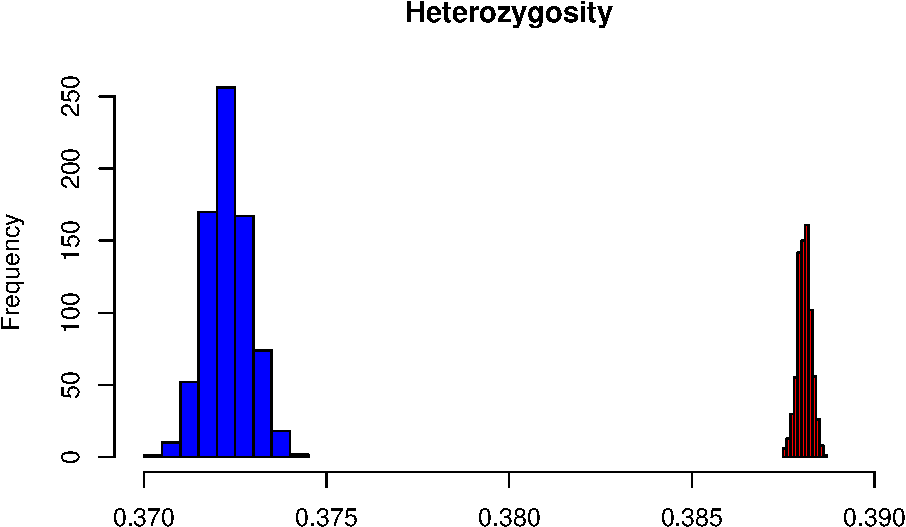
\includegraphics{supplement_files/figure-latex/unnamed-chunk-4-1.pdf}

\begin{Shaded}
\begin{Highlighting}[]
\CommentTok{# Calculate summary stats (mean and 95% highest posterior density [HPD] interval)}
\CommentTok{# with the quantile() function.}
\KeywordTok{list}\NormalTok{(}\StringTok{"mean_exp"} \NormalTok{=}\StringTok{ }\KeywordTok{mean}\NormalTok{(multi_het_exp), }
     \StringTok{"95HPD_exp"} \NormalTok{=}\StringTok{ }\KeywordTok{quantile}\NormalTok{(multi_het_exp, }\KeywordTok{c}\NormalTok{(}\FloatTok{0.025}\NormalTok{, }\FloatTok{0.975}\NormalTok{)), }
     \StringTok{"mean_obs"} \NormalTok{=}\StringTok{ }\KeywordTok{mean}\NormalTok{(multi_het_obs), }
     \StringTok{"95HPD_obs"} \NormalTok{=}\StringTok{ }\KeywordTok{quantile}\NormalTok{(multi_het_obs, }\KeywordTok{c}\NormalTok{(}\FloatTok{0.025}\NormalTok{, }\FloatTok{0.975}\NormalTok{)))}
\end{Highlighting}
\end{Shaded}

\begin{verbatim}
## $mean_exp
## [1] 0.3722944
## 
## $`95HPD_exp`
##      2.5%     97.5% 
## 0.3711756 0.3735096 
## 
## $mean_obs
## [1] 0.3880829
## 
## $`95HPD_obs`
##      2.5%     97.5% 
## 0.3877001 0.3884551
\end{verbatim}

As can be seen from the histograms and the summary statistics, the
observed heterozygosity is higher than the expected heterozygosity,
consistent with a pattern of inbreeding.

\subsection{\texorpdfstring{\emph{Evaluating model
adequacy}}{Evaluating model adequacy}}\label{evaluating-model-adequacy}

To evaluate model adequacy using posterior predictive simulation, we
used the posterior distribution of allele frequencies from the
\textsc{polyfreqs} run (\texttt{potato\_mcmc.out}) minus burn-in to look
at model fit on a per locus basis. You will also need the original read
count data to compare the observed and predicted read count ratios for
each locus.

\begin{Shaded}
\begin{Highlighting}[]
\CommentTok{# Read in the original read cound data using read.table().}
\CommentTok{# Again, remember the row.names and header arguments.}
\NormalTok{potato_tot_table <-}\StringTok{ }\KeywordTok{read.table}\NormalTok{(}\StringTok{"potato_tot_reads.txt"}\NormalTok{, }\DataTypeTok{row.names=}\DecValTok{1}\NormalTok{, }\DataTypeTok{header=}\NormalTok{T)}
\NormalTok{potato_ref_table <-}\StringTok{ }\KeywordTok{read.table}\NormalTok{(}\StringTok{"potato_ref_reads.txt"}\NormalTok{, }\DataTypeTok{row.names=}\DecValTok{1}\NormalTok{, }\DataTypeTok{header=}\NormalTok{T)}

\CommentTok{# If you haven't done so, load polyfreqs.}
\KeywordTok{library}\NormalTok{(polyfreqs)}

\CommentTok{# Now we'll read in the posterior distribution of allele frequencies.}
\NormalTok{potato_mcmc_table <-}\StringTok{ }\KeywordTok{read.table}\NormalTok{(}\StringTok{"potato_mcmc.out"}\NormalTok{, }\DataTypeTok{row.names=}\DecValTok{1}\NormalTok{, }\DataTypeTok{header=}\NormalTok{T)}

\CommentTok{# Take burn-in}
\NormalTok{potato_post <-}\StringTok{ }\NormalTok{potato_mcmc_table[}\DecValTok{251}\NormalTok{:}\DecValTok{1000}\NormalTok{,]}

\CommentTok{# Check for convergence}
\KeywordTok{sum}\NormalTok{(}\KeywordTok{effectiveSize}\NormalTok{(}\KeywordTok{mcmc}\NormalTok{(potato_post)) <}\StringTok{ }\DecValTok{200}\NormalTok{)}
\end{Highlighting}
\end{Shaded}

\begin{verbatim}
## [1] 0
\end{verbatim}

\begin{Shaded}
\begin{Highlighting}[]
\KeywordTok{plot}\NormalTok{(}\KeywordTok{mcmc}\NormalTok{(potato_post[,}\DecValTok{4}\NormalTok{]))}
\end{Highlighting}
\end{Shaded}

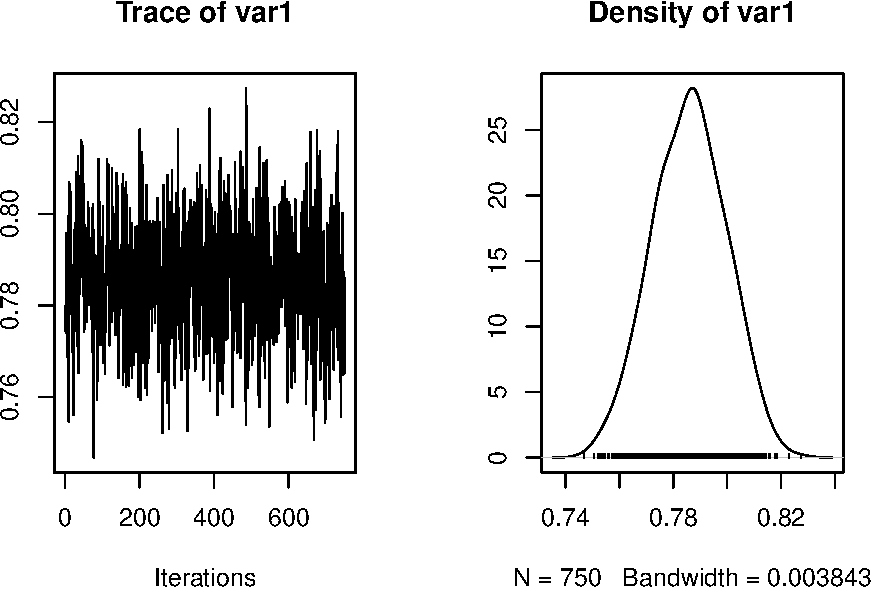
\includegraphics{supplement_files/figure-latex/unnamed-chunk-5-1.pdf}

\begin{Shaded}
\begin{Highlighting}[]
\CommentTok{# Run the analysis using the polyfreqs_pps() function.}
\NormalTok{potato_pps <-}\StringTok{ }\KeywordTok{polyfreqs_pps}\NormalTok{(}\KeywordTok{as.matrix}\NormalTok{(potato_post), }
                            \KeywordTok{as.matrix}\NormalTok{(potato_tot_table), }
                            \KeywordTok{as.matrix}\NormalTok{(potato_ref_table), }
                            \DataTypeTok{ploidy=}\DecValTok{4}\NormalTok{, }\DataTypeTok{error=}\FloatTok{0.01}\NormalTok{)}
\end{Highlighting}
\end{Shaded}

The \texttt{potato\_pps} object will be a list with two items:

\begin{itemize}
\item
  \texttt{potato\_pps\$ratio\_diff} -- A matrix with the per locus
  posterior predictive samples of the read ratio differences.
\item
  \texttt{potato\_pps\$locus\_fit} -- A logical vector indicating
  whether each locus passed or failed the posterior predictive check.
\end{itemize}

These two items can then be used to examine various aspects of model fit
such as the proportion of adequate/inadequate loci and plotting the
posterior predictive distribuion of read ratio differences for
inadequate loci.

\begin{Shaded}
\begin{Highlighting}[]
\CommentTok{# Get the proportion of adequate and inadequate loci.}
\KeywordTok{list}\NormalTok{(}\StringTok{"adequate"} \NormalTok{=}\StringTok{ }\KeywordTok{mean}\NormalTok{(potato_pps$locus_fit), }
     \StringTok{"inadequate"} \NormalTok{=}\StringTok{ }\DecValTok{1} \NormalTok{-}\StringTok{ }\KeywordTok{mean}\NormalTok{(potato_pps$locus_fit))}
\end{Highlighting}
\end{Shaded}

\begin{verbatim}
## $adequate
## [1] 0.8697917
## 
## $inadequate
## [1] 0.1302083
\end{verbatim}

\begin{Shaded}
\begin{Highlighting}[]
\CommentTok{# Get the names of the loci that are inadequate (provided that locus names are given).}
\KeywordTok{names}\NormalTok{(potato_pps$locus_fit[potato_pps$locus_fit==}\OtherTok{FALSE}\NormalTok{])}
\end{Highlighting}
\end{Shaded}

\begin{verbatim}
##  [1] "PotSNP002" "PotSNP015" "PotSNP020" "PotSNP044" "PotSNp071"
##  [6] "PotSNP080" "PotSNP104" "PotSNP138" "PotSNP140" "PotSNP154"
## [11] "PotSNP183" "PotSNP193" "PotSNP213" "PotSNP225" "PotSNP236"
## [16] "PotSNP238" "PotSNP245" "PotSNP247" "PotSNP249" "PotSNP252"
## [21] "PotSNP254" "PotSNP258" "PotSNP259" "PotSNP262" "PotSNP267"
## [26] "PotSNP268" "PotSNP275" "PotSNP277" "PotSNP286" "PotSNP287"
## [31] "PotSNP289" "PotSNP299" "PotSNP300" "PotSNP310" "PotSNP311"
## [36] "PotSNP313" "PotSNP327" "PotSNP329" "PotSNP331" "PotSNP335"
## [41] "PotSNP339" "PotSNP360" "PotSNP367" "PotSNP368" "PotSNP369"
## [46] "PotSNP372" "PotSNP373" "PotSNP377" "PotSNP383" "PotSNP384"
\end{verbatim}

\begin{Shaded}
\begin{Highlighting}[]
\CommentTok{# plot the posterior predictive distribution of read ratio differences.}
\NormalTok{inadequate <-}\StringTok{ }\KeywordTok{names}\NormalTok{(potato_pps$locus_fit[potato_pps$locus_fit==}\OtherTok{FALSE}\NormalTok{])}
\KeywordTok{hist}\NormalTok{(potato_pps$ratio_diff[,inadequate[}\DecValTok{1}\NormalTok{]], }\DataTypeTok{main=}\NormalTok{inadequate[}\DecValTok{1}\NormalTok{], }\DataTypeTok{xlab=}\StringTok{""}\NormalTok{)}
\end{Highlighting}
\end{Shaded}

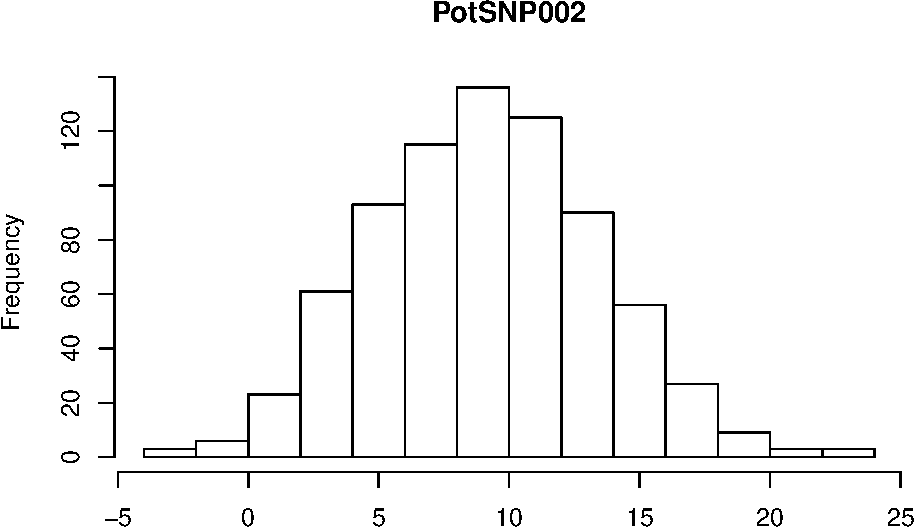
\includegraphics{supplement_files/figure-latex/unnamed-chunk-6-1.pdf}

The stochastic nature of simulating data may change the results between
posterior predictive model checking runs slightly, but we consistently
get \textasciitilde{}13-14\% of loci fitting the model poorly.

\beginsupplement

\begin{figure}[b]
\centering
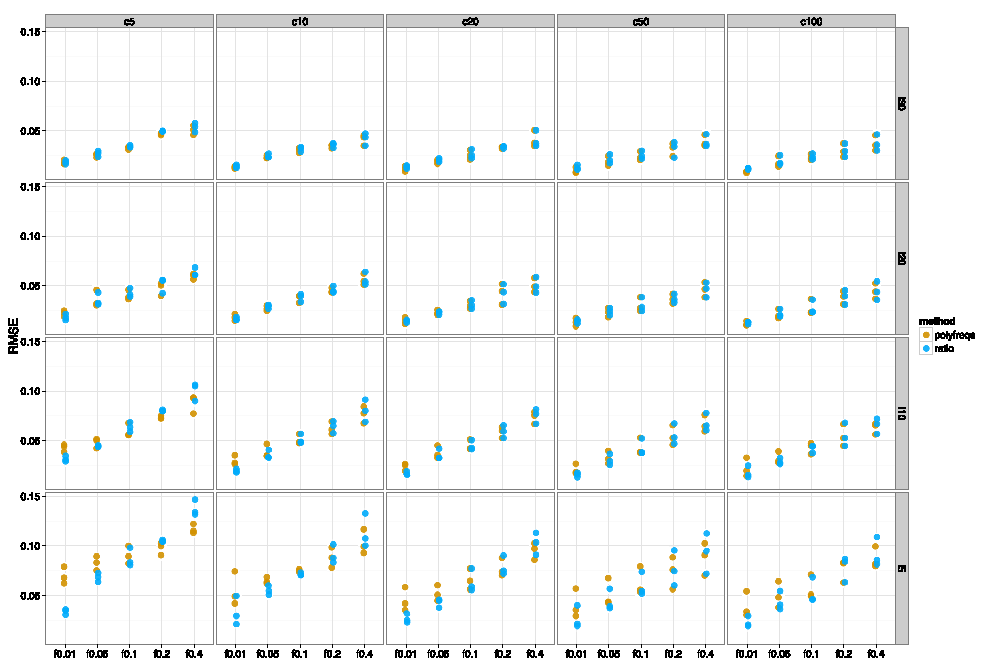
\includegraphics[width=\textwidth]{pdf/figS1}
\caption{Comparison of posterior mean versus simple mean read ratio estimates of allele frequencies for all simulation settings. All panels are set up the same as in Figure 1.}
\end{figure}



\begin{figure}[b]
\centering
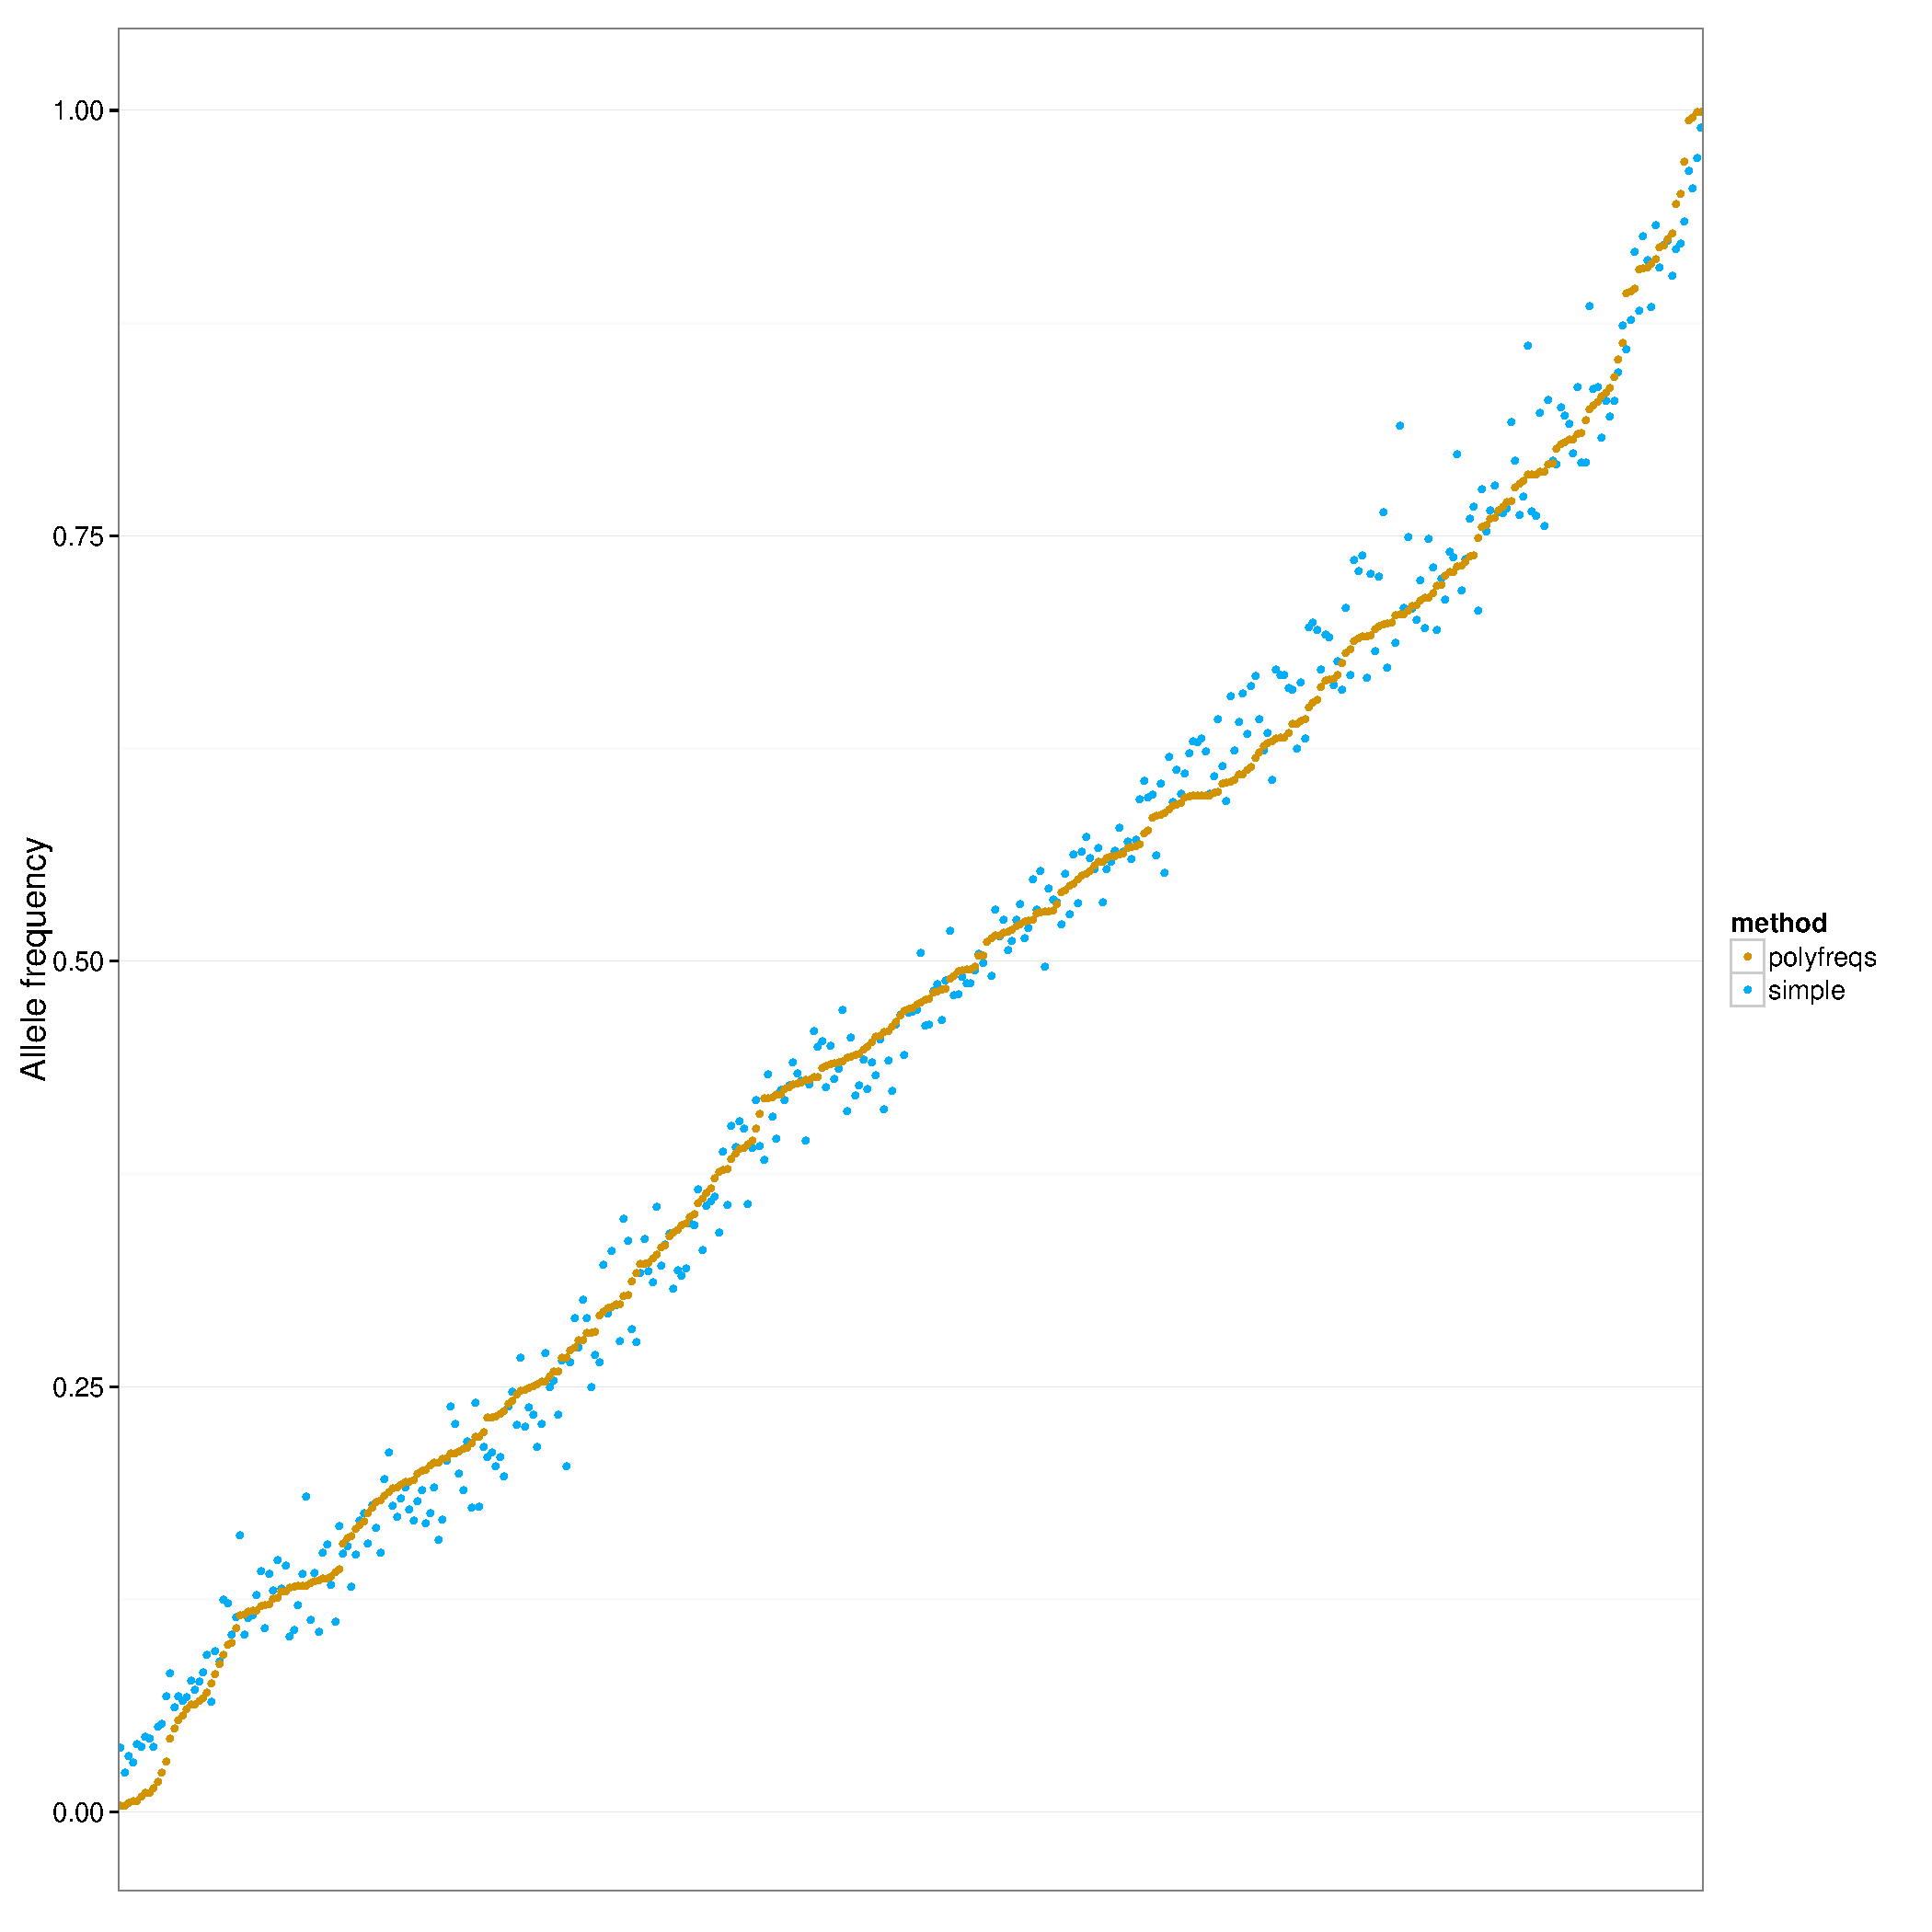
\includegraphics[width=\textwidth]{pdf/figS2}
\caption{Comparison of posterior mean versus simple mean read ratio estimates of allele frequencies for \textit{Solanum tuberosum}. We sorted the estimates from lowest to highest based on the posterior mean, which is why the simple estimates appear to be quite stochastic. The same result is seen in the posterior mean estimates if the results are sorted by the simple estimate.}
\end{figure}



\begin{figure}[b]
\centering
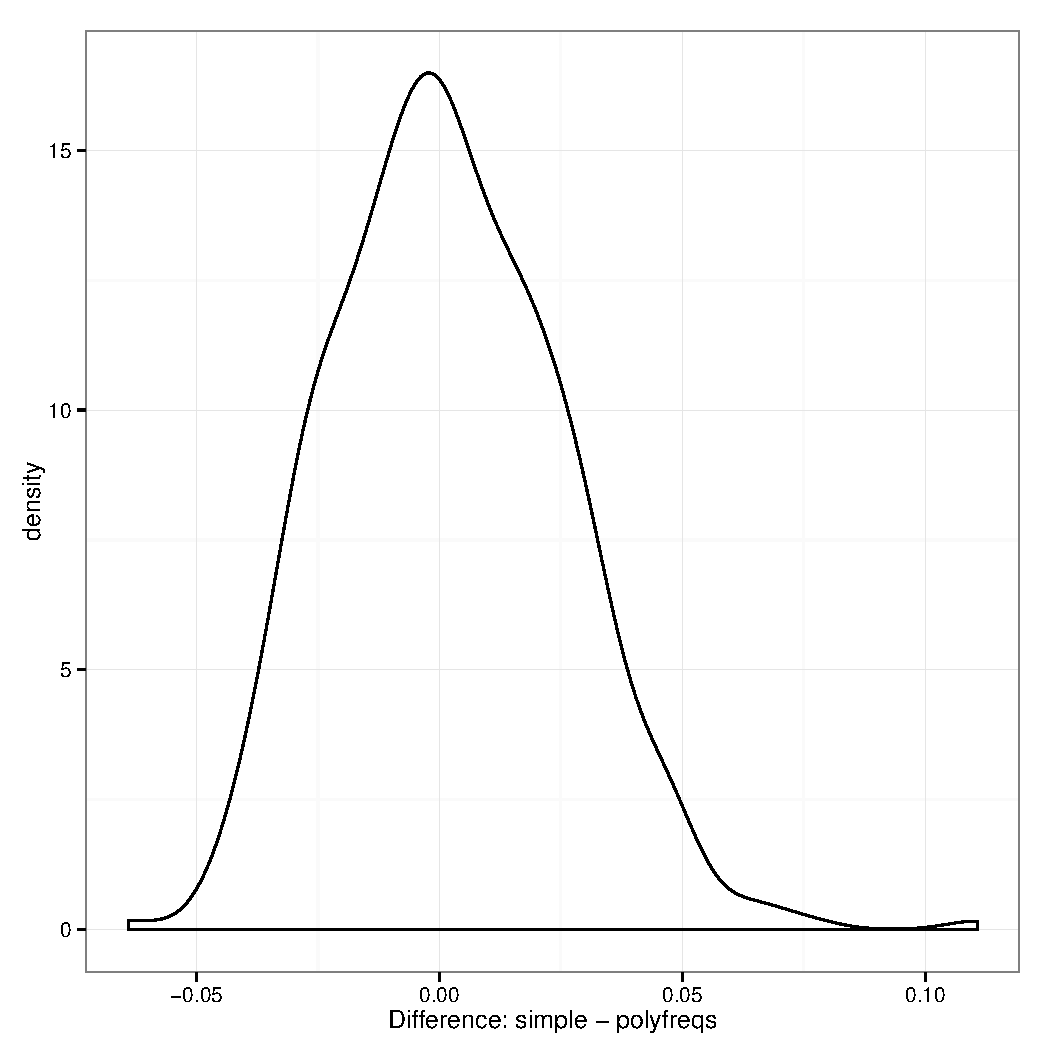
\includegraphics[width=0.6\textwidth]{pdf/figS3}
\caption{Density plot of the difference between the posterior mean and simple allele frequency estimate in \textit{Solanum tuberosum} taken for all loci.}
\end{figure}

\end{document}
